\section{Implementation}

The algorithms were implemented in RTL (VHDL) for use in an FPGA or ASIC.
The demodulator was also implemented in C. 
It turns out that with a little effort, the C and VHDL versions are in the same
order of magnitude of performance when comparing desktop CPU core to FPGA.
The RTL is faster, but not way faster.

The RTL uses a CORDIC-based FFT with a throughput of about 7 clocks per sample.
Since the FFT dominates the processing time, downsampling and upsampling
are performed when the FFT is idle.
This allows single-port RAM access and sharing of the CORDIC hardware. 
All buffers are single-port RAM for the sake of die size.
Overall throughput for a demodulator is about 12 clocks per input sample,
so about 10 MSPS. The input sample rate (such as from an ADC) is that divided
by the oversampling factor. For example, 100x oversampling results in
an ADC sample rate of 100 kSPS.

\begin{figure}
	\centering
	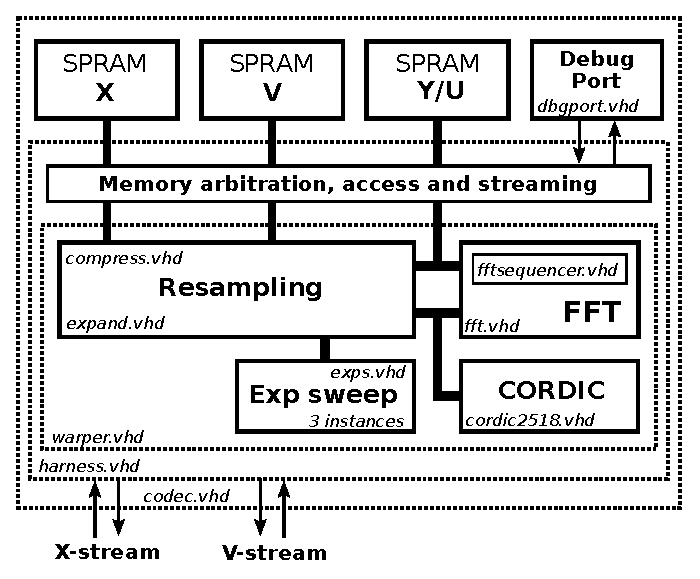
\includegraphics[width=0.8\linewidth]{../source/rtl_e}
	\caption[Quantum Time to Relative Time Hardware]{RTL Block Diagram}
	\label{fig:rtl}
\end{figure}

\subsection{Instrumentation}

The test port uses a half-duplex byte-oriented streaming protocol to access
hardware features for testing, verification, and debugging.
If necessary, the I/O streams may also be handled through the test port.
It uses all byte codes between 00 and FF, except for 10 to 13,
which are reserved for embedded ``escape sequences'' and flow control.
This strategy allows for XON/XOFF flow control if a UART is used as the PHY.
The PHY may be a USB FIFO chip (such as FT232H), SPI, UART, JTAG, or TWI.

The test port is used with test apps to verify separate steps of the
algorithm such as downsample, FFT, upsample, etc.
Connection to a test PC through a 2-wire UART is sufficient for FPGA testing.
The entire transform is coded in vanilla VHDL for ease of porting.

The demodulator/modulator shown in Fig.~\ref{fig:rtl} uses three memory
spaces to allow easier I/O access by the I/O streams and account for the
difference in word widths between X and V data.
The \verb|warper| uses wide data busses on the X and V memories to facilitate
correlation of outgoing data using long accumulators in either X or V memory.
Incoming data is packed two points per memory word.

\subsection {FPGA utilization}

A complete CODEC was implemented in vanilla VHDL with a single clock domain.
Free versions of synthesis tools were used to synthesize the design for use in
some sample FPGAs.
The clock rate is limited by the exponential sweep module,
which uses a single-cycle feedback loop whose path includes a 26x27 multiplier,
4:1 mux, adder, and 3:1 mux. Those two muxes will do better on FPGAs with
6-input LUTs. Synthesis for parts with LUT6 had a 50\% reduction in LUT usage
compared to LUT4-only.

Quartus Prime Pro fit six cores into a 10CX105YU484I6G (20$\mu$m FPGA),
with a power dissipation of about 5.8 watts at 100 MHz.
A system with 6 or 8 cores could be cooled with a small fan heat sink combo.

\begin{table}[t]\centering
	\label{tab:FPGAfit}
	\caption{FPGA rough synthesis results. One-off distributor pricing gives a
	rough cost per MHz, using Digikey pricing, across the number of CODEC
	instances that will fit in the FPGA.}
	\centering
	\begin{tabular}{lccrrr}
		\hline\hline
		Device & Logic & DSPs & Clock & Cores & \$/MHz\\ [0.5ex]
		\hline
        Artix 7     & 8K LUT6 & 40   & 100 MHz & 12 & 0.16\\
		Cyclone 10GX& 38K ALM & 125  & 100 MHz &  6 & 0.21\\
		LFE5        & 12K LE  & 40    & 39 MHz &  1 & 0.30\\
        PolarFire   & 14K LUT4 & 37   & 51 MHz &  7 & 0.40\\
		Cyclone 5   & 5K ALM & 18     & 72 MHz &  2 & 0.55\\
		MAX10       & 13K LE & 69 9x9 & 51 MHz &  1 & 1.20\\
		\hline
	\end{tabular}
\end{table}

